\documentclass[10pt]{article}
%----------Packages----------
\usepackage[utf8]{inputenc}
\usepackage[landscape,left=5mm,right=5mm,top=5mm,bottom=5mm]{geometry}
\usepackage{amsmath,amssymb}
\usepackage{siunitx}
\usepackage{multicol}
\usepackage{multirow}
\usepackage{blindtext}
\usepackage{graphicx}
\usepackage[e]{esvect} % https://ctan.mirror.globo.tech/macros/latex/contrib/esvect/esvect.pdf
\sisetup{per-mode=symbol}

%----------Page formatting----------
\pagenumbering{gobble}
% \everymath{\displaystyle}
\setlength{\parindent}{0pt}
% \setlength{\parskip}{2pt}
\renewcommand\labelitemi{$\vcenter{\hbox{\tiny$\bullet$}}$}

%----------Symbols----------
\newcommand{\ep}{\varepsilon}

%----------General----------
\newcommand{\ds}{\displaystyle}
\newcommand{\tab}{\hspace{.02\textwidth}}
\newcommand{\twoEqn}[4]{$\makebox[#3][l]{$#1$} \makebox[#4][l]{$#2$}$}
\newcommand{\threeEqn}[6]{$\makebox[#4][l]{$#1$} \makebox[#5][l]{$#2$} \makebox[#6][l]{$#3$}$}
\newcommand{\fourEqn}[8]{$\makebox[#5][l]{$#1$} \makebox[#6][l]{$#2$} \makebox[#7][l]{$#3$} \makebox[#8][l]{$#4$}$}
\newcommand{\splittab}{\hspace{2.58ex}}

%----------Math----------
\renewcommand{\d}{\,\mathrm{d}}
\newcommand{\p}{\partial}
\newcommand{\dv}[2]{\frac{d #1}{d #2}}
\newcommand{\ddv}[2]{\frac{d^2 #1}{d #2^2}}
\newcommand{\pd}[2]{\frac{\partial #1}{\partial #2}}
\newcommand{\pdd}[2]{\frac{\partial^2 #1}{\partial #2^2}}
\newcommand{\inv}{^{-1}}
\newcommand{\grad}{\nabla}
\newcommand{\lap}{\grad^2}
\newcommand{\Z}{\mathbb Z}

%----------Brackets----------
\newcommand{\lrb}[1]{\left(#1\right)}
\newcommand{\sqb}[1]{\left[#1\right]}
\newcommand{\abs}[1]{\left|#1\right|}
\newcommand{\set}[1]{\left\{#1\right\}}
\let\originalleft\left
\let\originalright\right
\renewcommand{\left}{\mathopen{}\mathclose\bgroup\originalleft}
\renewcommand{\right}{\aftergroup\egroup\originalright}


%----------Sections----------
\makeatletter
\renewcommand{\section}{\@startsection{section}{1}{0ex}
                                {-1ex}
                                {0.7ex}
                                {\normalfont\large\bfseries}}
\renewcommand{\subsection}{\@startsection{subsection}{2}{0ex}
                                {-0.4ex}
                                {0.4ex}
                                {\normalfont\normalsize\bfseries}}
\makeatother
\setcounter{secnumdepth}{0}

%----------PHYS 250----------
\newcommand{\cross}{\times}
\newcommand{\bs}{\boldsymbol}
\newcommand{\bv}[1]{\mathbf{#1}}

\newcommand{\moving}{\text{moving}}
\newcommand{\rest}{\text{rest}}
\newcommand{\obs}{\text{obs}}
\newcommand{\source}{\text{source}}

\newcommand{\rel}{\text{rel}}
\newcommand{\CM}{\text{CM}}
\renewcommand{\stop}{\text{stop}}
\newcommand{\tube}{\text{tube}}
\newcommand{\surface}{\text{surface}}
\newcommand{\normal}{\text{normal}}

\newcommand{\bohr}{\text{bohr}}
\newcommand{\photon}{\text{photon}}
\newcommand{\electron}{\text{electron}}
\newcommand{\matter}{\text{matter}}

% Vector and 4-Vector
\renewcommand{\vec}{\vv}

\DeclareFontFamily{U}{matha}{\hyphenchar\font45}
\DeclareFontShape{U}{matha}{m}{n}{<5><6><7><8><9><10> gen*matha}{}
\DeclareSymbolFont{matha}{U}{matha}{m}{n}
\DeclareMathSymbol{\varrightharpoonup}{3}{matha}{"E1}
\DeclareMathSymbol{\varrightharpoondown}{3}{matha}{"E3}

\makeatletter
\newcommand{\fourVec}{\mathpalette{\underarrow@\rightharpoondownfill@}}
\newcommand{\rightharpoondownfill@}{\arrowfill@\relbar\relbar\varrightharpoondown}
\makeatother


%----------Document Begins Here----------
\begin{document}

\begin{multicols*}{3}
\raggedcolumns

{\LARGE{\underline{PHYS 250 Formula Sheet}}}

\section{Constants}

$\SI{1}{\eV}=\SI{1.602e-19}{\J}$

$q=\SI{1.602e-19}{\C}$

$c=\SI{2.998e8}{\m\per\s}$

$h=\SI{6.626e-34}{\J\s}=\SI{4.136e-15}{\eV\s}$

$hc=\SI{1240}{\eV\nm}=\SI{1.986e-25}{\J\m}$

$\hbar=\frac{h}{2\pi}=\SI{1.055e-34}{\J\s}=\SI{6.5821e-16}{\eV\s}$

$k=\SI{1.381e-23}{\J\per\K}=\SI{8.617e-5}{\eV\per\K}$

$m_e=\SI{9.11e-31}{\kg}=\SI{0.511}{\MeV}/c^2$

$m_p=\SI{1.673e-27}{\kg}=\SI{938.3}{\MeV}/c^2$

\section{Relativity}

\subsection{Lorentz Transforms}

{\renewcommand{\arraystretch}{1.4}
\begin{tabular}{@{}ll}
    Lorentz Factor & $\beta=\frac uc=\sqrt{1-\frac{1}{\gamma^2}}$ \\ 
    & $\gamma=\frac{1}{\sqrt{1-\beta^2}}$ \\
    Approximations & \twoEqn{\gamma\approx 1+\frac 12\beta^2}{(\beta\ll 1)}{8em}{6em} \\
    & \twoEqn{\beta\approx 1-\frac 12\gamma^{-2}}{(\gamma\gg 1)}{8em}{6em} \\
    Transforms & \twoEqn{x'=\gamma(x-\beta ct)}{ct'=\gamma(ct-\beta x)}{8em}{6em} \\
    Inverse Transforms & \twoEqn{x=\gamma(x'+\beta ct')}{ct=\gamma(ct'+\beta x')}{8em}{6em} \\
    Time Dilation & $T_\moving=\gamma T_\rest$ \\
    Length Contraction & $L_\moving=\frac{L_\rest}{\gamma}$ \\
    Velocity Addition & $\beta=\frac{\beta_1+\beta_2}{1+\beta_1\beta_2}$ \\
    Doppler Effect & $f_\obs=f_\source\sqrt{\frac{1-\beta}{1+\beta}}$ \\
    & $\beta>0\iff$ distance increasing
\end{tabular}}

\subsection{Relativistic Energy-Momentum}

{\renewcommand{\arraystretch}{1.4}
\begin{tabular}{@{}ll}
    4-Vector & $\fourVec X=\lrb{ct,x,y,z}=\lrb{ct,\vec x}$ \\
    Dot Product & $\fourVec{X_1}\cdot\fourVec{X_2}=(ct_1)(ct_2)-\vec{x_1}\cdot\vec{x_2}$ \\
    Rel Mass & $M=\gamma m$ \\
    Kinetic & $K=(\gamma-1)mc^2$ \\
    Rel Momentum & $p=\gamma mv$ \\
    Rel Energy & $E=\gamma mc^2$ \\
    & $E^2=(pc)^2+(mc^2)^2$ \\
    Transforms & \twoEqn{E'=\gamma(E-\beta cp)}{p'=\gamma(p-\beta cE)}{9em}{6em} \\
    Inverse & \twoEqn{E=\gamma(E'+\beta cp')}{p=\gamma(p'+\beta cE')}{9em}{6em} \\
    4-Momentum & \twoEqn{\fourVec P=\lrb{\frac{E_\rel}{c},\vec{p_\rel}}}{\fourVec P^2=(mc)^2}{9em}{6em} \\
    CM Energy & $E_\CM=(\fourVec{P_1}+\fourVec{P_2})^2$ \\ 
    & $\phantom{E_\CM}=m_1^2+2\fourVec{P_1}\cdot\fourVec{P_2}+m_2^2$
\end{tabular}}

\section{Photons}

{\renewcommand{\arraystretch}{1.4}
\begin{tabular}{@{}ll}
    Types of Light & UV: $100-\SI{400}{\nm}$ \\
    & Visible: $400-\SI{750}{\nm}$ \\
    & IR: $750-\SI{1000}{\nm}$ \\
    Photon Energy & $E=hf=\frac{hc}{\lambda}$ \\
    Photon Momentum & $p=\frac Ec=\frac h\lambda$ \\
    RJ Blackbody & $dI_{RJ}(f)=\frac{2kTf^2}{c^2}df$ \\
    & $dI_{RJ}(\lambda)=\frac{2kTc}{\lambda^4}d\lambda$ \\
    Wien Blackbody & $dI_W(f)=\frac{2hf^3}{c^2}\exp\bigl(-\frac{hf}{kT}\bigr)df$ \\
    & $dI_W(\lambda)=\frac{2hc^2}{\lambda^5}\exp\bigl(-\frac{hc}{\lambda kT}\bigr)d\lambda$ \\
    Planck Blackbody & $dI_P(f)=\frac{2hf^3}{c^2}\frac{1}{\exp\lrb{\frac{hf}{kT}}-1}df$ \\ 
    & $dI_P(\lambda)=\frac{2hc^2}{\lambda^5}\frac{1}{\exp\lrb{\frac{hc}{\lambda kT}}-1}d\lambda$ \\
    Photoelectric & $qV_{\stop}=E_{k,\max}=hf-\phi q$ \\
    X-ray Tube & $qV_{\tube}(+q\phi)=hf_{\max}=\frac{hc}{\lambda_{\min}}$ \\
    Compton Scattering & $\lambda'-\lambda=\frac{h}{mc}(1-\cos\theta)$ \\
    & $\frac{h}{mc}=\SI{2.426}{\pm}$ \\
    Plane Diffraction & $2d\sin(\theta_\surface)=n\lambda$ \\
    Slit Diffraction & $d\sin(\theta_\normal)=n\lambda$
\end{tabular}}

\section{Atoms}

{\renewcommand{\arraystretch}{1.4}
\begin{tabular}{@{}ll}
    Rydberg & $\frac{1}{\lambda}=RZ^2\bigl(\frac{1}{n_1^2}-\frac{1}{n_2^2}\bigr)$ \\
    & $R=\SI[per-mode=reciprocal]{1.097e7}{\per\m}$ \\
    Photon Energy & $E=\SI{13.6}{\eV}\cdot Z^2\bigl(\frac{1}{n_1^2}-\frac{1}{n_2^2}\bigr)$ \\
    Orbit Energy & $E=-\frac 12\frac{q^2Z}{4\pi\epsilon_0}\frac 1r=-Z\cdot\frac{\SI{0.7202}{\eV\nm}}{r}$ \\
    Bohr Model & $L=n\hbar$ \\
    Bohr Energy & $E=-\frac{m_e}{2}\bigl(\frac{q^2}{4\pi\epsilon_0\hbar}\bigr)^2\frac{Z^2}{n^2}=\SI{-13.6}{\eV}\bigl(\frac{Z^2}{n^2}\bigr)$ \\
    Bohr Radius & $r=\frac{4\pi\epsilon_0\hbar^2n^2}{Zmq^2}=\SI{52.97}{\pico\meter}\bigl(\frac{n^2}{Z}\bigr)$ \\
    Bohr Velocity & \twoEqn{v=\frac{Zq^2}{4\pi\ep_0n\hbar}}{\beta=\num{7.293e-3}\bigl(\frac Zn\bigr)}{7em}{9em} \\
    Moseley's Law & $E=\SI{13.6}{\eV}\bigl(\frac{1}{n_1^2}-\frac{1}{n_2^2}\bigr)(Z-b)^2$ \\
    & ${\begin{aligned}
        &\mathrm{K}\alpha\colon &&b=1,&n_1=1,&&n_2=2 \\
        &\mathrm{K}\beta\colon &&b=1,&n_1=1,&&n_2=3 \\
        &\mathrm{L}\alpha\colon &&b=7.4,&n_1=2,&&n_2=3
    \end{aligned}}$ \\
    De Broglie & $p=\frac Ec=\frac{hf}{c}=\frac{h}{\lambda_\photon}$ \\
    & $\lambda_{\electron}=\frac{\SI{1.227}{\sqrt{eV}\cdot\nm}}{\sqrt{E_{k,\electron}}}$ \\
    & $\lambda_{\matter}=\frac{h}{\sqrt{2mE_k}}$
\end{tabular}}

\section{1-D Schrodinger}

{\renewcommand{\arraystretch}{1.4}
\begin{tabular}{@{}ll}
    Wavefunction & $\Psi(x,t)$ \\
    Equation & $i\hbar\pd{\Psi}{t}=-\frac{\hbar^2}{2m}\pdd{\Psi}{x}+V(x)\Psi=H_{op}\Psi$ \\
    Hamiltonian & $H_{op}=-\frac{\hbar^2}{2m}\pdd{}{x}+V(x)$ \\
    Free Particle & $\Psi(x,t)=Ae^{i(kx-\omega t)}$ \\
    & \fourEqn{k=\frac{2\pi}{\lambda}}{\lambda=\frac hp}{\omega=2\pi f}{f=\frac Eh}{4em}{4em}{5em}{5em} \\
    & \twoEqn{p=\hbar k}{E=\hbar\omega}{8em}{10em} \\
    Separation & $\Psi(x,t)=\psi(x)\phi(t)$ \\
    Time-Dependent & $\phi(t)=e^{-iEt/\hbar}$ \\
    TISE & $-\frac{\hbar^2}{2m}\ddv{\psi}{x}+V(x)\psi=E\psi$ \\ 
    Probability & $\rho(x)=\Psi^*\Psi\qquad \int_{-\infty}^\infty\Psi^*\Psi\,dx=1$ \\
    Gaussian & $f(x)=\frac{1}{\sqrt{2\pi\sigma^2}}e^{-\frac{x^2}{2\sigma^2}}$ \\
    Transform & $\sigma_x\sigma_k=1$ \\
    Uncertainty & $\sigma_x\sigma_p\ge\frac{\hbar}{2}$
\end{tabular}}

\subsection{Potential Step}

{\renewcommand{\arraystretch}{1.4}
\begin{tabular}{@{}ll}
    Wavefunctions & $\begin{cases}
        \psi_I=e^{ikx} &\text{(Incident)} \\
        \psi_R=Re^{-ikx} &\text{(Reflected)} \\
        \psi_T=Te^{ik'x} &\text{(Transmitted)}
    \end{cases}$ \\
    Wavenumbers & \twoEqn{k=\frac{\sqrt{2mE}}{\hbar}}{k'=\frac{\sqrt{2m(E-V)}}{\hbar}}{9em}{8em} \\
    Amplitudes & \twoEqn{R=\frac{k-k'}{k+k'}}{T=\frac{2k}{k+k'}}{9em}{8em} \\
    & \twoEqn{R=\frac{\sqrt{E}-\sqrt{E-V}}{\sqrt{E}+\sqrt{E-V}}}{T=\frac{2\sqrt{E}}{\sqrt{E}+\sqrt{E-V}}}{9em}{8em} \\
    Flux & $\Phi=\rho\cdot v$ \\
    & \twoEqn{\Phi_I=\frac{\hbar k}{m}}{\Phi_I=\Phi_R+\Phi_T}{9em}{8em} \\
    & \twoEqn{\Phi_R=\frac{\hbar k}{m}R^2}{\Phi_T=\frac{\hbar k'}{m}T^2}{9em}{8em} \\ 
    Probabilities & \twoEqn{P(R)=\frac{\Phi_R}{\Phi_I}=R^2}{P(T)=\frac{\Phi_T}{\Phi_I}=\frac{k'}{k}T^2}{9em}{8em}
\end{tabular}}

\subsection{Potential Barrier}
Wavefunctions 
$\quad\begin{cases}
    \psi_I=e^{ikx} &\text{(Incident)} \\
    \psi_R=Re^{-ikx} &\text{(Reflected)} \\
    \psi_T=Te^{ikx} &\text{(Transmitted)} \\
    \psi_F=Fe^{ik'x} &\text{(Forward)} \\
    \psi_B=Be^{-ik'x} &\text{(Backward)}
\end{cases}$

$\begin{bmatrix}
    -1 & 1 & 1 & 0 \\
    k & k' & -k' & 0 \\
    0 & e^{ik'w} & e^{-ik'w} & -e^{ikw} \\
    0 & k'e^{ik'w} & -k'e^{-ik'w} & -ke^{ikw}
\end{bmatrix}
\begin{bmatrix} R \\ F \\ B \\ T\end{bmatrix}=
\begin{bmatrix} 1 \\ k \\ 0 \\ 0\end{bmatrix}$

{\renewcommand{\arraystretch}{1.4}
\begin{tabular}{@{}ll}
    Tunneling & $P(T)\approx 16\frac EV(1-\frac EV)e^{-2\kappa w}$ \\ 
    & $\kappa=\frac{\sqrt{2m(V-E)}}{\hbar}$
\end{tabular}}

\subsection{Infinite Square Well}

{\renewcommand{\arraystretch}{1.4}
\begin{tabular}{@{}ll}
    Energy & $E_n=\frac{\hbar^2\pi^2}{2m}\frac{n^2}{w^2}$ \\
    & $\frac{\hbar^2\pi^2}{2m_e}=\SI{0.37603}{\eV\nm}$ (for electron) \\
    Inside & \twoEqn{\psi_n(x)=\sqrt{\frac 2w}\sin(k_n x)}{k_n=\frac{n\pi}{w}}{15em}{4em} \\
    Outside & \twoEqn{\psi_n(x)=e^{\pm k'x}}{k_n'=\frac{n\pi}{w}}{15em}{4em}
\end{tabular}}

\subsection{Finite Potential Wells}

{\renewcommand{\arraystretch}{1.4}
\begin{tabular}{@{}ll}
    Energy & $E_n\approx\frac{\hbar^2\pi^2n^2}{2mw^2}-V, \quad E<0$ \\
    Inside & \twoEqn{\psi_n(x)=A\sin(kx)+B\cos(kx)}{k=\frac{\sqrt{2mE}}{\hbar}}{15em}{4em} \\
    Outside & \twoEqn{\psi_n(x)=Ce^{k'x}+De^{-k'x}}{k'=\frac{\sqrt{2m(V-E)}}{\hbar}}{12.7em}{6em} \\
\end{tabular}}

\subsection{Quantum Harmonic Oscillator}

{\renewcommand{\arraystretch}{1.4}
\begin{tabular}{@{}ll}
    Potential & $V(x)=\frac 12k'x^2$ \\
    Energy & \twoEqn{E_n=\lrb{n+\frac 12}\hbar\omega}{\omega=\sqrt{\frac{k'}{m}}}{12em}{5em} \\
    Wavefunction & \twoEqn{\psi_n(x)=H_n(\frac xb)e^{-\frac{x^2}{2b^2}}}{b^2=\frac{\hbar}{\sqrt{k'm}}}{12em}{5em} \\
    Hermite & \twoEqn{H_0(x)=1}{H_1(x)=x}{8em}{8em} \\
    & \twoEqn{H_2(x)=x^2-\frac 12}{H_3(x)=x^3-\frac 32x}{8em}{8em}
\end{tabular}}

\section{3-D Schrodinger}

{\renewcommand{\arraystretch}{1.4}
\begin{tabular}{@{}ll}
    Wavefunction & $\Psi(x,y,z,t)=\Psi(\vec x,t)$ \\
    Laplacian & $\lap\Psi(x,y,z)=\pdd \Psi x+\pdd \Psi y+\pdd \Psi z$ \\
    Equation & $i\hbar\pd{\Psi}{t}=-\frac{\hbar^2}{2m}\lap\Psi+V(\vec x)\Psi$ \\
    Free Particle & $\Psi(\vec x,t)=Ae^{i(\vec k\cdot\vec x-\omega t)}$ \\
    & \twoEqn{\vec p=\hbar\vec k}{E=\hbar\omega}{8em}{8em} \\ 
    Separation & $\Psi(\vec x,t)=\psi(\vec x)\phi(t)$ \\
    Time-Dependent & $\phi(t)=e^{-iEt/\hbar}$ \\
    TISE & $-\frac{\hbar^2}{2m}\lap\psi+V(\vec x)\psi=E\psi$
\end{tabular}}

\subsection{Infinite Box Well}

{\renewcommand{\arraystretch}{1.4}
\begin{tabular}{@{}ll}
    Energy & $E_{n_x,n_y,n_z}=\bigl(\frac{n_x^2}{a^2}+\frac{n_y^2}{b^2}+\frac{n_z^2}{c^2}\bigr)\frac{\hbar^2\pi^2}{2m}$ \\
    Cube & $E_{n_x,n_y,n_z}=(n_x^2+n_y^2+n_z^2)\frac{\hbar^2\pi^2}{2m}\frac{1}{w^2}$ \\
    Wavefunction & $\psi_{\vec n}(x,y,z)=\sin(\frac{n_x\pi x}{a})\sin(\frac{n_y\pi y}{b})\sin(\frac{n_z\pi z}{c})$
\end{tabular}}

\subsection{Spherical Coordinates}

$\lap\Psi=\frac{1}{r^2}\pd{}{r}\sqb{r^2\pd \Psi r}+\frac{1}{r^2\sin\theta}\pd{}{\theta}\sqb{\sin\theta\pd\Psi\theta}+\frac{1}{r^2\sin^2\theta}\pdd\Psi\phi$
{\renewcommand{\arraystretch}{1.4}
\begin{tabular}{@{}ll}
    Separation & $\psi(r,\theta,\phi)=F(r)G(\theta)H(\phi)$ \\
    Equations & $\begin{cases}
        \pdd{H(\phi)}{\phi}=-\mu H(\phi) \\
        \sin\theta\pd{}{\theta}\sqb{\sin\theta\pd{G(\theta)}{\theta}}=(\mu-\lambda\sin^2\theta)G(\theta) \\
        -\frac{\hbar^2}{2M}\pdd{U(r)}{r}+\sqb{V(r)+\frac{\hbar^2\lambda}{2Mr^2}U(r)}=EU(r)
    \end{cases}$ \\
    Solutions & $H(\phi)=e^{im\phi}, m\in\Z$ \\
    & $G(\theta)=P_l^m(\theta)$ (Legendre functions) \\
    & $F(r)=\frac 1rU_{kl}(r)$ \\
    Harmonics & $Y_l^m(\theta,\phi)=P_l^m(\theta)e^{im\phi}$ \\ 
    General & $\psi_{klm}(r,\theta,\phi)=\frac{1}{r}U_{kl}(r)Y_l^m(\theta,\phi)$
\end{tabular}}

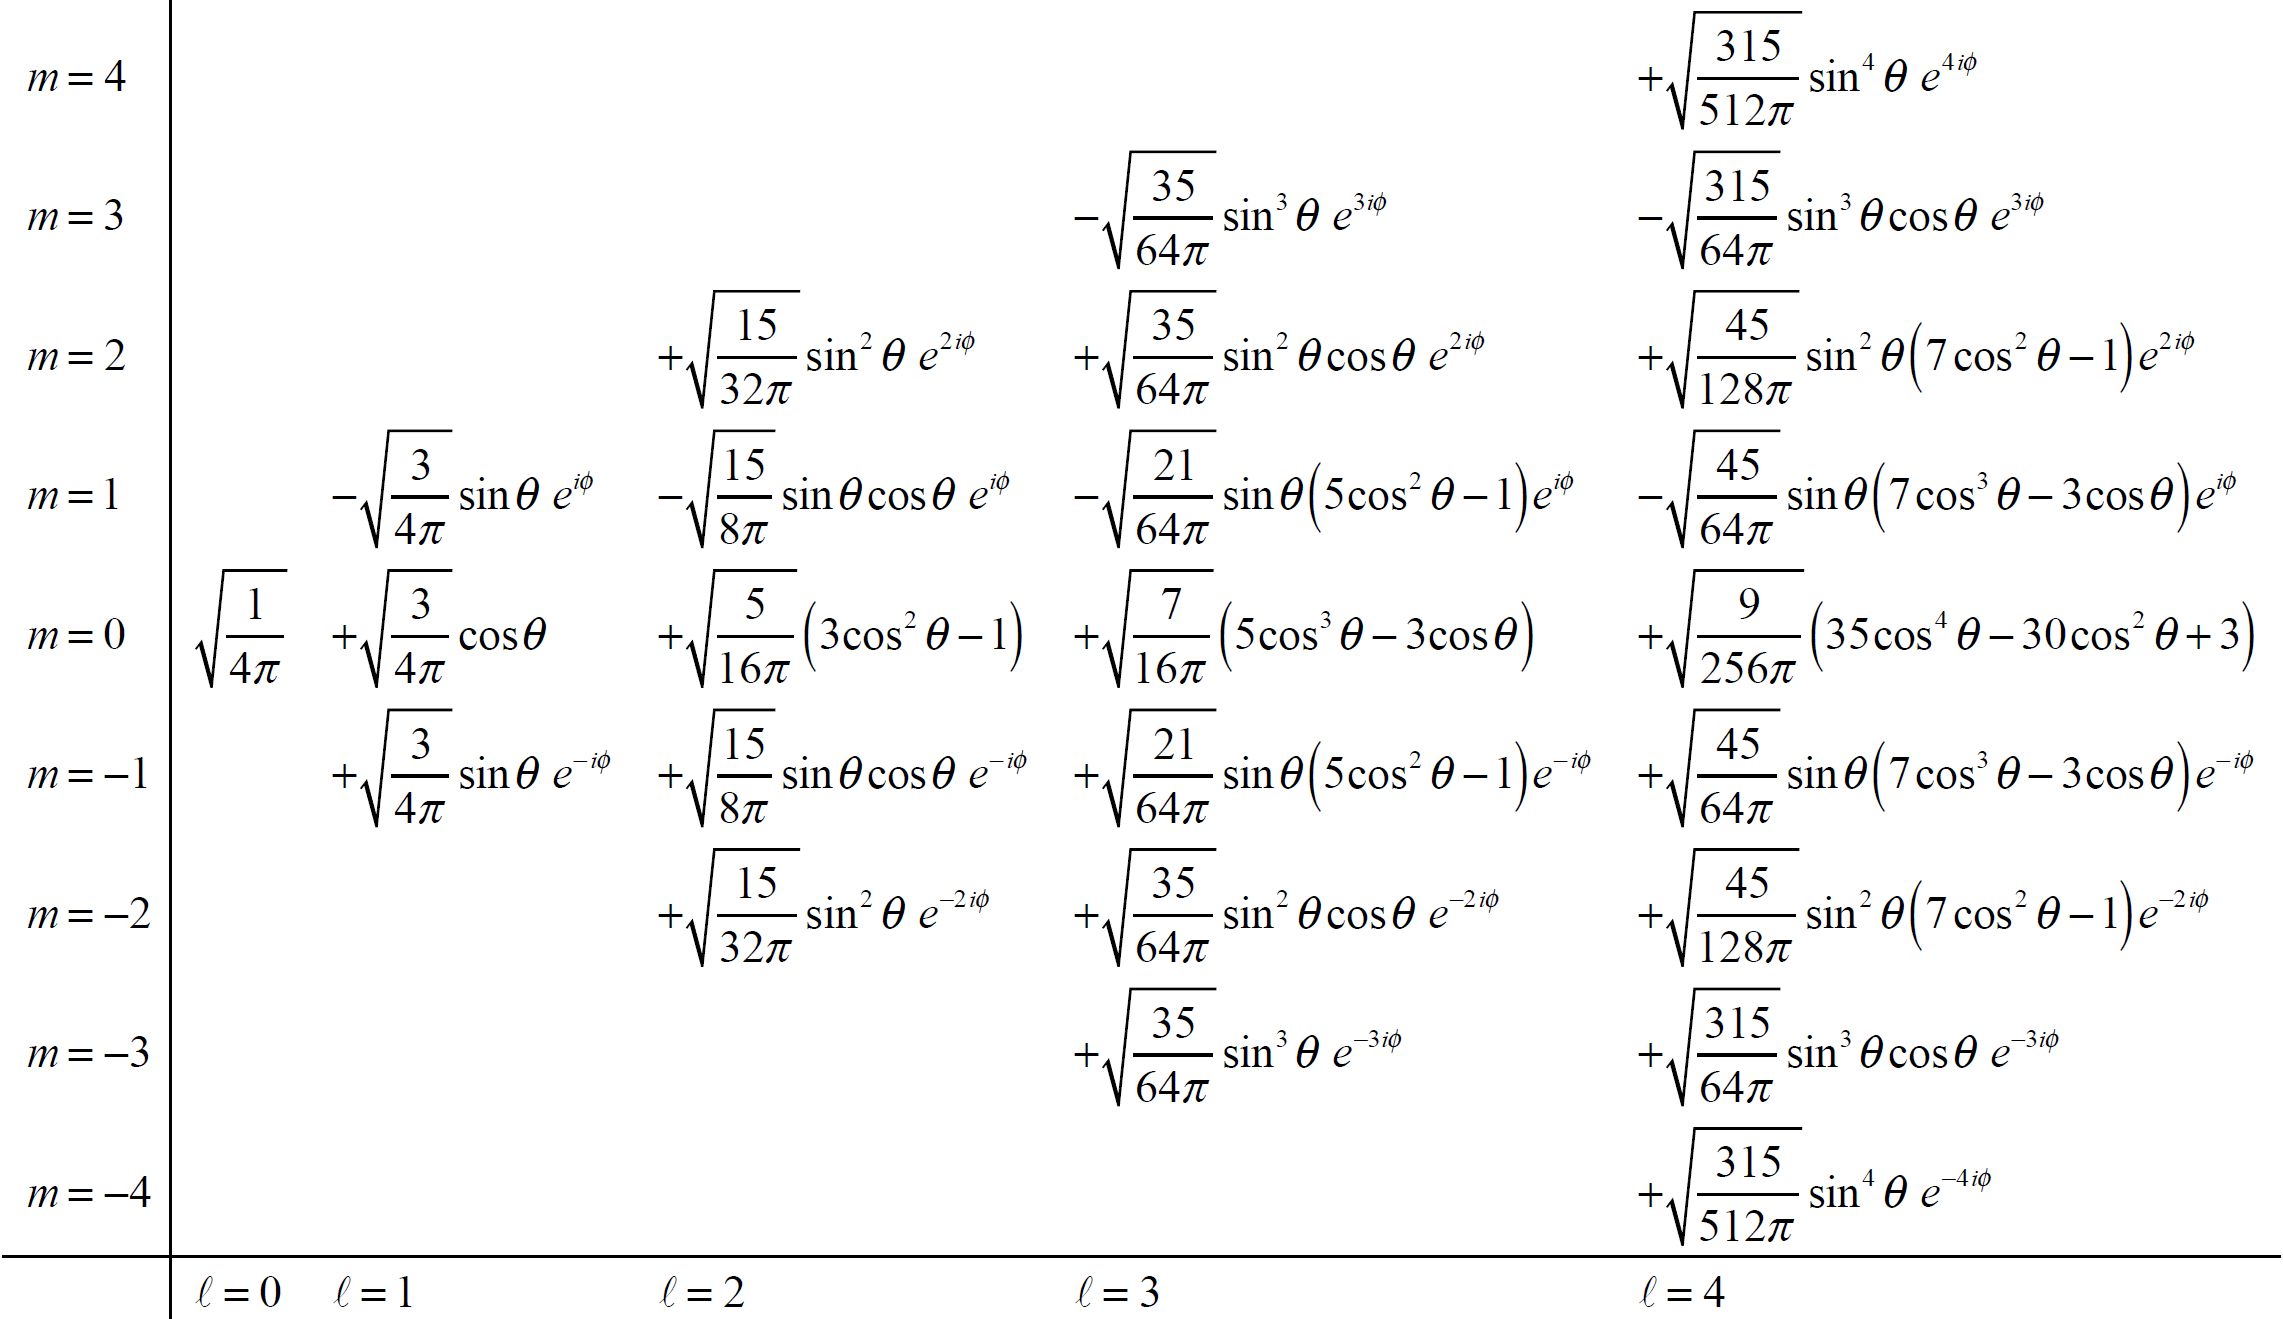
\includegraphics[width=\linewidth]{images/spherical_harmonics.png}

{\renewcommand{\arraystretch}{1.4}
\begin{tabular}{@{}ll}
    Angular & $l=\set{0,1,2,\ldots}$ \\
    Magnetic & $m=\set{\ldots,-1,0,1,\ldots},\quad\abs{m}\le l$ \\
    Radial & $k\in\Z$, starting from $0$ or $1$ \\
    Principal & $n=k+l$ (for $\frac 1r$ potential) \\
    & $\lambda=l(l+1)$
\end{tabular}}

\subsection{Infinite Spherical Well}

{\renewcommand{\arraystretch}{1.4}
\begin{tabular}{@{}ll}
    Energy & $E_{k0}=\frac{\hbar^2\pi^2}{2M}\frac{k^2}{R^2}$ \\
    Wavefunction & $U_{k0}(r)=\sin\bigl(\frac{k\pi r}{R}\bigr)$ \\
    & $\psi_{k00}=\frac 1r\sin\bigl(\frac{k\pi r}{R}\bigr)Y_0^0(\theta,\phi)=\frac 1r\sin\bigl(\frac{k\pi r}{R}\bigr)$
\end{tabular}}

\subsection{Infinite Shell}

{\renewcommand{\arraystretch}{1.4}
\begin{tabular}{@{}ll}
    Energy & $E_{kl}=\frac{\hbar^2\pi^2}{2M}\sqb{\frac{k^2}{\Delta R^2}+\frac{l(l+1)}{\pi^2(R+\Delta R/2)^2}}$ \\
    Centrifugal Term & $\frac{\hbar^2l(l+1)}{2M(R+\Delta R/2)^2}\approx\frac{\hbar^2 l(l+1)}{2MR^2} \quad (\Delta R\ll R)$ \\
    Wavefunction & $U_{k0}(r)=\sin\bigl(\frac{k\pi(r-R)}{\Delta R}\bigr)$ \\
    & $\psi_{k00}=\frac 1r\sin\bigl(\frac{k\pi(r-R)}{\Delta R}\bigr)$
\end{tabular}}

\subsection{Coulomb Potential and Hydrogen}

{\renewcommand{\arraystretch}{1.4}
\begin{tabular}{@{}ll}
    Potential & $V(r)=-\frac{q^2}{4\pi\ep_0r}$ \\
    Wavefunction & $\psi_{nlm}(r,\theta,\phi)=e^{-\frac{\rho}{2}}\rho^l L_{n-l-1}^{2l+1}(\rho)Y_l^m(\theta,\phi)$ \\ 
    & \twoEqn{\rho=\frac{2r}{na_0}}{a_0=\SI{52.97}{\pm}}{8em}{5em}
\end{tabular}}

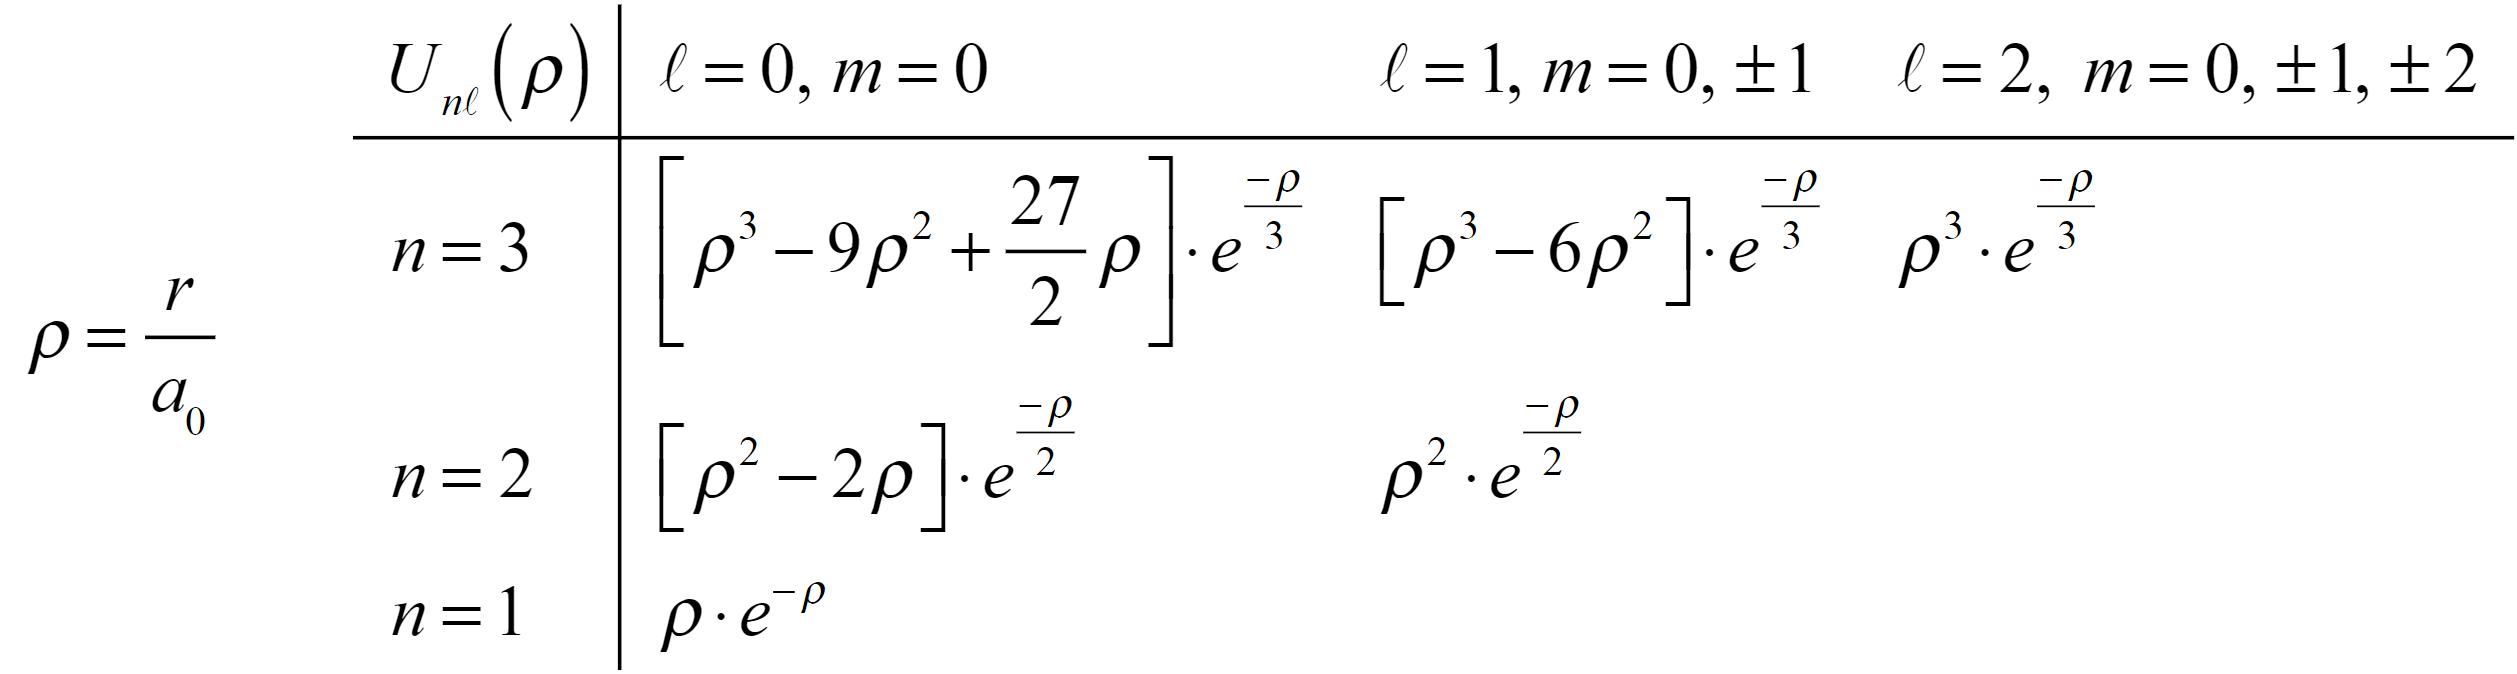
\includegraphics[width=\linewidth]{images/hydrogen_radial_wavefunction.png}

{\renewcommand{\arraystretch}{1.4}
\begin{tabular}{@{}ll}
    Principal & $\exp\bigl(-\frac{r}{na_0}\bigr)\implies n$ \\
    Angular & $\sin$ power $+$ max $\cos$ power $\implies l$ \\
    Magnetic & $\exp(im\phi)\implies m$
\end{tabular}}

\rule{\linewidth}{0.1pt}

\scriptsize 
Compiled \today

\end{multicols*}

\end{document}